% Copyright 2016 by Till Alamgir Hossain

\documentclass{beamer}

% There are many different themes available for Beamer. 
%\usetheme{AnnArbor}
%\usetheme{Antibes}
%\usetheme{Bergen}
%\usetheme{Berkeley}
%\usetheme{Berlin}
%\usetheme{Boadilla}
%\usetheme{boxes}
\usetheme{CambridgeUS}
%\usetheme{Copenhagen}
%\usetheme{Darmstadt}
%\usetheme{default}
%\usetheme{Frankfurt}
%\usetheme{Goettingen}
%\usetheme{Hannover}
%\usetheme{Ilmenau}
%\usetheme{JuanLesPins}
%\usetheme{Luebeck}
%\usetheme{Madrid}
%\usetheme{Malmoe}
%\usetheme{Marburg}
%\usetheme{Montpellier}
%\usetheme{PaloAlto}
%\usetheme{Pittsburgh}
%\usetheme{Rochester}
%\usetheme{Singapore}
%\usetheme{Szeged}
%\usetheme{Warsaw}

\title{Quadratic Equations}

% A subtitle is optional and this may be deleted
\subtitle{equation, roots, plots}

\author{Alamgir Hossain}
%\author{F.~Author\inst{1} \and S.~Another\inst{2}}
% - Give the names in the same order as the appear in the paper.
% - Use the \inst{?} command only if the authors have different
%   affiliation.

\institute[] % (optional, but mostly needed)
  {
  Assistant Professor (on study leave)\\
  Department of Mathematics\\
  Jagannath University, Bangladesh}
% - Use the \inst command only if there are several affiliations.
% - Keep it simple, no one is interested in your street address.
\date{\today}
%\date{Conference Name, 2016}
% - Either use conference name or its abbreviation.
% - Not really informative to the audience, more for people (including
%   yourself) who are reading the slides online

\subject{Mathematics}
% This is only inserted into the PDF information catalog. Can be left
% out. 

% If you have a file called "university-logo-filename.xxx", where xxx
% is a graphic format that can be processed by latex or pdflatex,
% resp., then you can add a logo as follows:

%\pgfdeclareimage[height=0.5cm]{jnu-logo}{jnu-logo}
%\logo{\pgfuseimage{jnu-logo}}

% Delete this, if you do not want the table of contents to pop up at
% the beginning of each subsection:
\AtBeginSubsection[]
{
  \begin{frame}<beamer>{Outline}
    \tableofcontents[currentsection,currentsubsection]
  \end{frame}
}

% Let's get started
\begin{document}

\begin{frame}
  \titlepage
\end{frame}

\begin{frame}{Outline}
  \tableofcontents
  % You might wish to add the option [pausesections]
\end{frame}

\section{About quadratic equation and roots }    

\begin{frame}
  \frametitle{Quadratic Equations}
    When $a \ne 0$, quadratic equation \cite{anton2002calculus}
    $$ ax^2 + bx + c = 0 $$ has two roots and they are
    $$x = \frac{-b \pm \sqrt{b^2-4ac}}{2a}.$$
\end{frame}


\begin{frame}
  \frametitle{Type of Roots}

  \begin{block}{Discriminant}
    $$d = b^2-4ac$$
    \end{block}

  \begin{itemize}
  \item
    $d \ge 0$; roots are real
    \begin{itemize}
  \item
    $d > 0$; roots are real and distinct
  \item
    $d = 0$; roots are real and same
    \end{itemize}
  \item
    $d<0$; roots are complex
\end{itemize}

\end{frame}

\begin{frame}
  \frametitle{Vertex of Parabola}
  \[ \begin{array}{rcl}
    y & = & a x^{2}+bx+c\\
      & = & a\left(x^{2}+2\times\frac{b}{2a}x+\frac{c}{a}\right)\\
      & = & a\left(x+\frac{b}{2a}\right)^2 - \frac{b^2}{4a} + c
    \end{array}\]

   Vertex of the parabola, $y = f(x)$ is
   $\left(-\frac{b}{2a}, c - \frac{b^2}{4a}\right)$.
\end{frame}

\section{Roots of quadratic equation in a table}

\begin{frame}
  \frametitle{Table: Type of roots}\label{table-type-of-roots}
  \begin{center}
    \begin{tabular}{|l|l|}
      \hline
      $d = b^2-4ac$ & comment about roots\\
      \hline \hline
      $d>0$ & roots are real and distinct\\
      \hline
      $d = 0$ & roots are real and same\\
      \hline
      $d<0$ & roots are complex\\
      \hline
    \end{tabular}
  \end{center}
\end{frame}

\section{Plots}

\begin{frame}
  \frametitle{Plots of quadratic equations}
    \begin{figure}
    \centering
    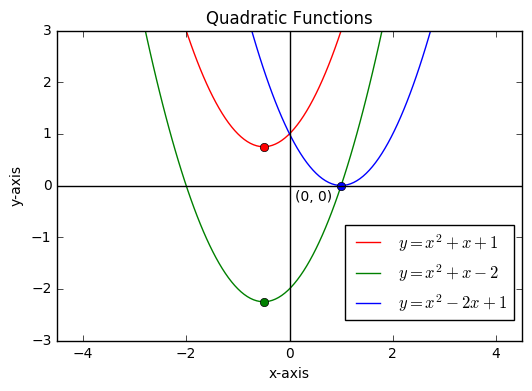
\includegraphics[scale=0.5]{quadraticplots.png}
    \caption{Quadratic Functions}
    \end{figure}
\end{frame}
 
\begin{frame}
  \frametitle{Reference}
    \bibliographystyle{unsrt}
    \bibliography{ref}
\end{frame}

\begin{frame}
    \centering
  Thank You!!!\\
  \vspace{1cm}
  Questions???
\end{frame}


\end{document}
